\documentclass[american,]{article}
\usepackage{lmodern}
\usepackage{amssymb,amsmath}
\usepackage{ifxetex,ifluatex}
\usepackage{fixltx2e} % provides \textsubscript
\ifnum 0\ifxetex 1\fi\ifluatex 1\fi=0 % if pdftex
  \usepackage[T1]{fontenc}
  \usepackage[utf8]{inputenc}
\else % if luatex or xelatex
  \ifxetex
    \usepackage{mathspec}
  \else
    \usepackage{fontspec}
  \fi
  \defaultfontfeatures{Ligatures=TeX,Scale=MatchLowercase}
\fi
% use upquote if available, for straight quotes in verbatim environments
\IfFileExists{upquote.sty}{\usepackage{upquote}}{}
% use microtype if available
\IfFileExists{microtype.sty}{%
\usepackage{microtype}
\UseMicrotypeSet[protrusion]{basicmath} % disable protrusion for tt fonts
}{}
\usepackage[margin=1in]{geometry}
\usepackage{hyperref}
\hypersetup{unicode=true,
            pdftitle={Regression Analysis of the Ames, Iowa Dataset},
            pdfauthor={Stuart Miller, Paul Adams, and Chance Robinson},
            pdfborder={0 0 0},
            breaklinks=true}
\urlstyle{same}  % don't use monospace font for urls
\ifnum 0\ifxetex 1\fi\ifluatex 1\fi=0 % if pdftex
  \usepackage[shorthands=off,main=american]{babel}
\else
  \usepackage{polyglossia}
  \setmainlanguage[variant=american]{english}
\fi
\usepackage{natbib}
\bibliographystyle{apalike}
\usepackage{longtable,booktabs}
\usepackage{graphicx,grffile}
\makeatletter
\def\maxwidth{\ifdim\Gin@nat@width>\linewidth\linewidth\else\Gin@nat@width\fi}
\def\maxheight{\ifdim\Gin@nat@height>\textheight\textheight\else\Gin@nat@height\fi}
\makeatother
% Scale images if necessary, so that they will not overflow the page
% margins by default, and it is still possible to overwrite the defaults
% using explicit options in \includegraphics[width, height, ...]{}
\setkeys{Gin}{width=\maxwidth,height=\maxheight,keepaspectratio}
\IfFileExists{parskip.sty}{%
\usepackage{parskip}
}{% else
\setlength{\parindent}{0pt}
\setlength{\parskip}{6pt plus 2pt minus 1pt}
}
\setlength{\emergencystretch}{3em}  % prevent overfull lines
\providecommand{\tightlist}{%
  \setlength{\itemsep}{0pt}\setlength{\parskip}{0pt}}
\setcounter{secnumdepth}{5}
% Redefines (sub)paragraphs to behave more like sections
\ifx\paragraph\undefined\else
\let\oldparagraph\paragraph
\renewcommand{\paragraph}[1]{\oldparagraph{#1}\mbox{}}
\fi
\ifx\subparagraph\undefined\else
\let\oldsubparagraph\subparagraph
\renewcommand{\subparagraph}[1]{\oldsubparagraph{#1}\mbox{}}
\fi

%%% Use protect on footnotes to avoid problems with footnotes in titles
\let\rmarkdownfootnote\footnote%
\def\footnote{\protect\rmarkdownfootnote}

%%% Change title format to be more compact
\usepackage{titling}

% Create subtitle command for use in maketitle
\newcommand{\subtitle}[1]{
  \posttitle{
    \begin{center}\large#1\end{center}
    }
}

\setlength{\droptitle}{-2em}

  \title{Regression Analysis of the Ames, Iowa Dataset}
    \pretitle{\vspace{\droptitle}\centering\huge}
  \posttitle{\par}
    \author{Stuart Miller, Paul Adams, and Chance Robinson}
    \preauthor{\centering\large\emph}
  \postauthor{\par}
      \predate{\centering\large\emph}
  \postdate{\par}
    \date{Master of Science in Data Science, Southern Methodist University, USA}

\usepackage{booktabs}
\usepackage{longtable}
\usepackage{array}
\usepackage{multirow}
\usepackage[table]{xcolor}
\usepackage{wrapfig}
\usepackage{float}
\usepackage{colortbl}
\usepackage{pdflscape}
\usepackage{tabu}
\usepackage{threeparttable}
\usepackage{threeparttablex}
\usepackage[normalem]{ulem}
\usepackage{makecell}

\usepackage{amsmath}
\usepackage[utf8]{inputenc}
\usepackage[T1]{fontenc}
\usepackage{setspace}
\usepackage{hyperref}
\onehalfspacing
\setcitestyle{numbers}
\newcommand\numberthis{\addtocounter{equation}{1}\tag{\theequation}}

\begin{document}
\maketitle

\hypertarget{introduction}{%
\section{Introduction}\label{introduction}}

\citet{Sleuth}

\hypertarget{ames-iowa-data-set}{%
\section{Ames, Iowa Data Set}\label{ames-iowa-data-set}}

The Ames, Iowa Data Set describes the sale of individual residential
properities from 2006-2010 in Ames, Iowa \cite{Cock}. The data was
retreved from the dataset hosting site Kaggle, where is it listed under
a machine learning competition named
\href{https://www.kaggle.com/c/house-prices-advanced-regression-techniques/overview}{\textit{House Prices: Advanced Regression Techniques}}
\cite{Kaggle2016}. The data is comprized of 37 numeric features, 43
non-numeric features and an obervation index split between a training
set and a testing set, which contain 1460 and 1459 observations,
respectively. The response variable (\texttt{SalePrice}) is only
provided for the training set. The output of a model on the test set can
be submitted to the Kaggle competition for scoring the performance of
the model in terms of RMSE. The first analysis models property sale
prices (\texttt{SalePrice}) as the response of living room area
(\texttt{GrLivArea}) of the property and neighborhood
(\texttt{Neighborhood}) where it is located. \textbf{Add some details on
the question 2 variables?}

\hypertarget{analysis-question-i}{%
\section{Analysis Question I}\label{analysis-question-i}}

\hypertarget{question-of-interest}{%
\subsection{Question of Interest}\label{question-of-interest}}

Century 21 has commissioned an analysis of this data to determine how
the sale price of property is related to living room area of the
property in the Edwards, Northwest Ames, and Brookside neighborhoods of
Ames, IA.

\hypertarget{modeling}{%
\subsection{Modeling}\label{modeling}}

Linear regression will be used to model sale price as a response of the
living room area. From the intial exploratory data analysis, it was
determined that sale prices should be log transformed to meet the model
assumptions \textbf{Add appendix reference}. Additionally, two
observations were removed as they appeared to be from a different
population than the other observations in the dataset \textbf{Add
appendix reference}.

We will consider two models: the logarithm of sale price as the response
of living room area (1), the reduced model, and the logarithm of sale
price as the response of living room area accounting for differences in
the three neighborhood of interest (Brookside, Northwest Ames, and
Edwards) where Edwards will be used as the reference (2), the full
model. An extra sums of square (ESS) test will be used to verify that
the addition of \texttt{Neighborhood} improves the model.

\textbf{Reduced Model}

\begin{equation}
\mu \lbrace log(SalePrice) \rbrace = \beta_0 + \beta_1(LivingRoomArea) \label{eq:reduced}
\end{equation}

\textbf{Full Model}

\begin{align}
\mu \lbrace log(SalePrice) \rbrace = \beta_0 + \beta_1(LivingRoomArea) +  \beta_2(Brookside) +\beta_3(NorthwestAmes) + \nonumber\\
\beta_3(Brookside)(LivingRoomArea) + \beta_4(NorthwestAmes)(LivingRoomArea) \label{eq:full}
\end{align}

The ESS test provides convincing evidence that the interaction terms are
useful for the model (p-value \textless{} 0.0001); thus, we will
continue with the full model.

\begin{verbatim}
## Analysis of Variance Table
## 
## Model 1: log(SalePrice) ~ (GrLivArea) + Neighborhood_BrkSide + Neighborhood_NAmes
## Model 2: log(SalePrice) ~ (GrLivArea) + Neighborhood_BrkSide + Neighborhood_NAmes + 
##     (GrLivArea) * Neighborhood_BrkSide + (GrLivArea) * Neighborhood_NAmes
##   Res.Df    RSS Df Sum of Sq      F    Pr(>F)    
## 1    377 14.824                                  
## 2    375 13.441  2    1.3834 19.299 1.053e-08 ***
## ---
## Signif. codes:  0 '***' 0.001 '**' 0.01 '*' 0.05 '.' 0.1 ' ' 1
\end{verbatim}

\hypertarget{model-assumptions-assessment}{%
\subsection{Model Assumptions
Assessment}\label{model-assumptions-assessment}}

The following assessments for model assumptions are made based on Figure
\ref{fig:diag-plots} and Figure 2 (\textbf{TODO}):

\begin{itemize}
\tightlist
\item
  The residuals of the model appear to be approximately normally
  distrubited based on the QQ plot of the residuals and histogram of the
  residuals, suggesting the assumption of normality is met.
\item
  No patterns are evident in the scatter plots of residuals and
  studentized residuals vs predicted value, suggesting the assumption of
  constant variance is met.
\item
  While some observations appear to be influential and have high
  leverage, removing these observations does not have a significant
  impact on the result of the model fit.
\item
  Based on the scatter plot of the log transform of \texttt{SalePrice}
  vs \texttt{GrLivArea}, it appears that a linear model is reasonable.
\end{itemize}

The sampling procedure is not known. We will assume the independence
assumption is met.

\begin{figure}[htbp]

{\centering 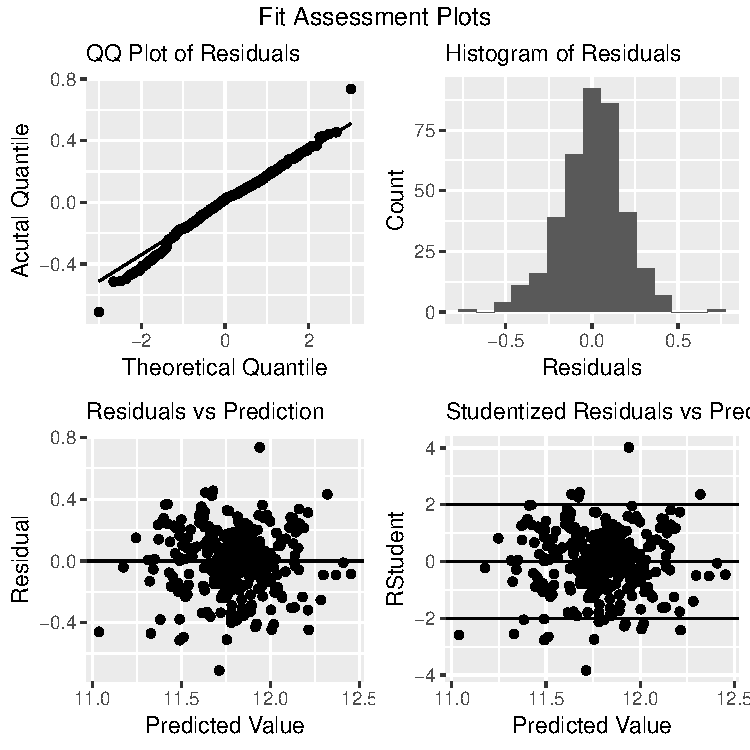
\includegraphics[width=0.45\linewidth]{HousePriceRegressionAnalysis_files/figure-latex/diag-plots-1} 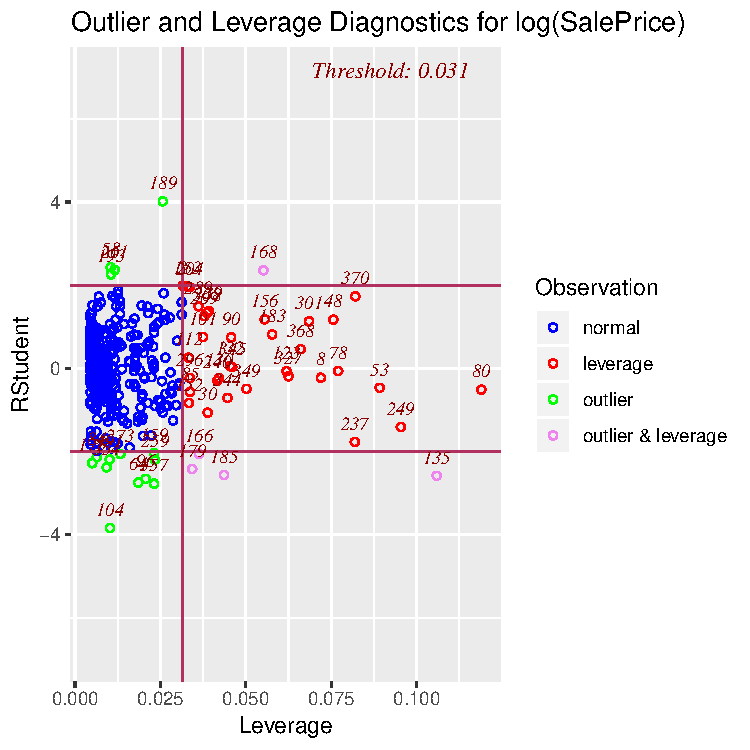
\includegraphics[width=0.45\linewidth]{HousePriceRegressionAnalysis_files/figure-latex/diag-plots-2} 

}

\caption{Diagnostic Plots}\label{fig:diag-plots}
\end{figure}

\hypertarget{comparing-competing-models}{%
\subsection{Comparing Competing
Models}\label{comparing-competing-models}}

The two models were trained and validated on the training dataset using
10-fold cross validation. The table below summerizes the performance of
the models with RMSE, adjusted \(R^2\), and PRESS. These results show
that the full model is an improvement over the reduced model, which is
consistent with the result of the ESS test.

\begin{table}[H]
\centering
\begin{tabular}{lrrr}
\toprule
Model & RMSE & CV.Press & Adjused.R.Squared\\
\midrule
Full Model & 0.1910566 & 12.51675 & 0.5084024\\
Reduced Model & 0.1988473 & 13.55835 & 0.4750767\\
\bottomrule
\end{tabular}
\end{table}

\hypertarget{parameters}{%
\subsection{Parameters}\label{parameters}}

\begin{itemize}
\tightlist
\item
  Estimates \textbf{TODO}
\item
  CI
\end{itemize}

\hypertarget{model-interpretation}{%
\subsection{Model Interpretation}\label{model-interpretation}}

We estimate that for increase in 100 sq. ft., there is associated
multiplicative increase in median price of

\begin{itemize}
\tightlist
\item
  1.055 for the Edwards neighborhood with a 95\% confidence interval of
  {[}1.044 , 1.066{]}
\item
  1.033 for the Northwest Ames neighorhood with a 95\% confidence
  interval of {[}1.026 , 1.040{]}
\item
  1.077 for the Brookside neighorhood with a 95\% confidence interval of
  {[}1.063 , 1.090{]}
\end{itemize}

Since the sampling procedure is not known and this is an observational
study, the results only apply to this data.

\hypertarget{conclusion}{%
\subsection{Conclusion}\label{conclusion}}

A short summary of the analysis

\hypertarget{analysis-question-ii}{%
\section{Analysis Question II}\label{analysis-question-ii}}

\hypertarget{question-of-interest-1}{%
\subsection{Question of Interest}\label{question-of-interest-1}}

Restatement of the problem

\hypertarget{modeling-1}{%
\subsection{Modeling}\label{modeling-1}}

Type of selection

\hypertarget{model-assumption-assessment}{%
\subsection{Model Assumption
Assessment}\label{model-assumption-assessment}}

Address each assumption

\hypertarget{comparing-competing-models-1}{%
\subsection{Comparing Competing
Models}\label{comparing-competing-models-1}}

\begin{itemize}
\tightlist
\item
  Adj \(R^2\)
\item
  CV Press
\item
  Kaggle score
\end{itemize}

\hypertarget{conclusion-1}{%
\subsection{Conclusion}\label{conclusion-1}}

A short summary of the analysis

\hypertarget{appendix}{%
\section{Appendix}\label{appendix}}

Include ``well commented'' \texttt{code} in the appendex!

\renewcommand\refname{References}
\bibliography{references.bib}


\end{document}
